\begin{itemize}
 \item Conceptual model
  \begin{figure}[h]
    \centering
    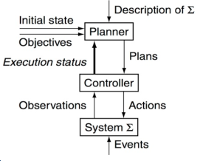
\includegraphics{./img/conceptual_model.png}
    \caption{Conceptual model}
  \end{figure}
 
 \item State-transition system
 
	$\Sigma = (S,A,E,\gamma)$
  \begin{itemize}
   \item $S$: states
   \item $A$: actions
   \item $E$: events
   \item $\gamma$: state-transition function
  \end{itemize} 	

 \item Objectives
 \begin{itemize}
  \item $S_g$: set of goal states
  \item utility function
 \end{itemize}
 
 \item Restrictive assumptions
 \begin{itemize}
  \item A0: finite $\sigma$
  \item A1: $\sigma$ is fully observable (observation function is id() )
  \item A2: deterministic $\sigma$, action: one possible outcome
  \item A3: static $\sigma$: E is empty
  \item A4: attainment goals: goal state or a set of goal states
  \item A5: sequential plans
  \item A6: implicit time (instant transitions)
  \item A7: off-line planning
 \end{itemize}
 
 \item Classical planning
 \begin{itemize}
  \item requires all eight restrictive assumptions
  \item Given $(\Sigma, s_0, S_g)$
  \item find a sequence of actions $<a_1,a_2,...,a_n>$
  \item that produces sequence of transitions $s_1 = \gamma(s_0,a_1), ...$
  \item such that $s_n \in S_g$
 \end{itemize}
 
 \item Relaxing assumptions
 \emph{Is this necessary?} 
 
\end{itemize}

